\documentclass[14pt]{extarticle}
\author{Jeon Yongjin, Kim Jaeyoung, Ju Minchan}
\usepackage{amsmath}
\usepackage{kotex}
\usepackage{graphicx}
\usepackage[margin=1in]{geometry} % Reduce margins to 1 inch
\title{\(_{Design}^{Capsonte}\) : 산업수학 프로젝트 정례 보고서}
\begin{document}
\maketitle

\section{\textit{What we have done}}

\subsection{작업 방향 설정}

이전 주차에 저희는 연구 주제에 익숙해지기 위해 관련 프로그램 학습 등을 진행하는 기초적인 이해 단계에 있었습니다.
저희의 최종적인 목표는 네트워크 트래픽 최적화 알고리즘 고안입니다. 
이를 위해서는 우선 트래픽을 분류하는 것이 우선시되어야 한다고 판단하였습니다.
분류의 기준에는 다양한 요소가 있을 수 있겠지만, 
우선적으로 클라이언트가 VPN을 통해 접속하는 경우와 VPN을 사용하지 않는 경우를 구분하는 것이 필요하다고 생각하였습니다.
이러한 분류를 통해 VPN을 사용하지 않는 클라이언트의 트래픽을 우선적으로 처리할 수 있는 알고리즘을 고안할 수 있을 것입니다.

\subsection{분류 모델 개발 - 데이터셋 선정 및 전처리}
데이터셋으로는 ISCX2016을 사용하였습니다.
이 데이터셋은 2016년 캐나다에서 수집된 트래픽 데이터로,
실제와 유사한 네트워크 환경에서 수집된 데이터이고, 다양한 프로토콜과 패턴 사용을 포함하고 있습니다.
또한 VPN을 사용하지 않는 클라이언트와 VPN을 사용하는 클라이언트의 트래픽을 포함하고 있기 때문에 라벨링된 데이터셋 지도학습 가능이 가능합니다.
저희는 이 데이터셋을 사용하여 VPN을 사용하지 않는 클라이언트의 트래픽을 분류하는 모델을 개발하였습니다.

ISSC2016 데이터셋에는 A1, A2, B의 3가지 시나리오가 존재하는데, 저희는 A1,A2 시나리오를 사용하였습니다.
B 시나리오는 VPN을 사용하지 않는 클라이언트의 트래픽을 포함하고 있지 않기 때문에 저희의 연구 주제와는 맞지 않다고 판단하여 제외하였습니다.
A2 시나리오에는 트래픽의 유형 (Browing, File Transfer, Streaming, VoIP 등)에 대한 정보가 포함되어 있기 때문에 활용하였습니다.
각 시나리오에는 15s, 30s, 60s, 120s의 시간 간격으로 수집된 트래픽 데이터가 포함되어 있고, 각 시간별 데이터의 양이 충분하다고 판단하여 60s의 데이터만을 사용하였습니다.

전처리 과정에서는 범주형 데이터(VPN/Non-VPN)를 수치형 데이터로 변환하는 작업을 진행하였습니다.
또한 데이터의 일부가 누락되어 있고, 중복 데이터가 존재하기 때문에 그에 대한 처리 또한 진행하였습니다.
마지막으로 IQR(Inter Quartile Range) 기법을 사용하여 이상치를 제거하였습니다. Figure 1에 전처리가 완료된 데이터의 크기 변화를 나타내었습니다.

\begin{figure}[h!]
    \centering
    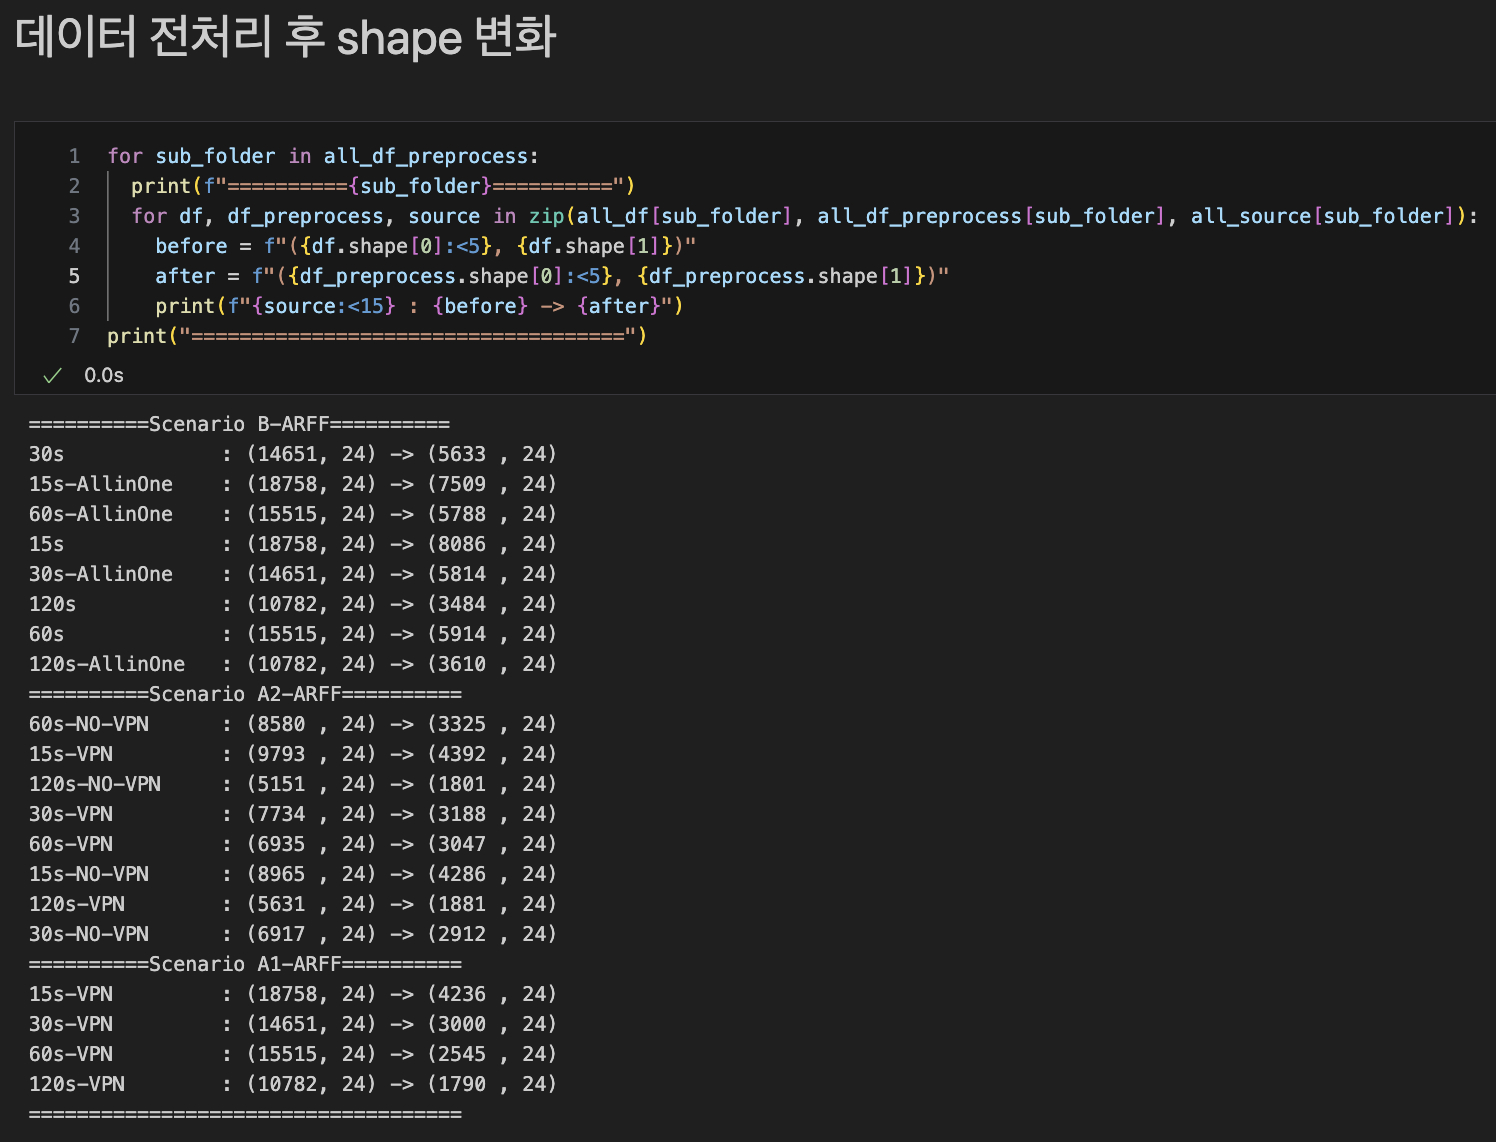
\includegraphics[width=0.8\textwidth]{Photo_Preprocessing} % 이미지 파일 이름
    \caption{전처리 결과}
\end{figure}

\subsection{분류 모델 개발 - 모델 학습}

모델 학습은 상관관계 분석과 xgboost를 사용하였습니다.
우선, 상관관계 분석을 통해 각 라벨과 VPN 사용 여부와의 상관관계를 분석하였습니다.
각 Heatmap으로 상관관계 분석을 통해 VPN 사용 여부와 상관관계가 어느 정도 존재하는 Label만을 남겼습니다.
상관관계 분석을 통해 남긴 Label과 그것의 Heatmap을 Figure 2에 나타내었습니다.

\begin{figure}[h!]
    \centering
    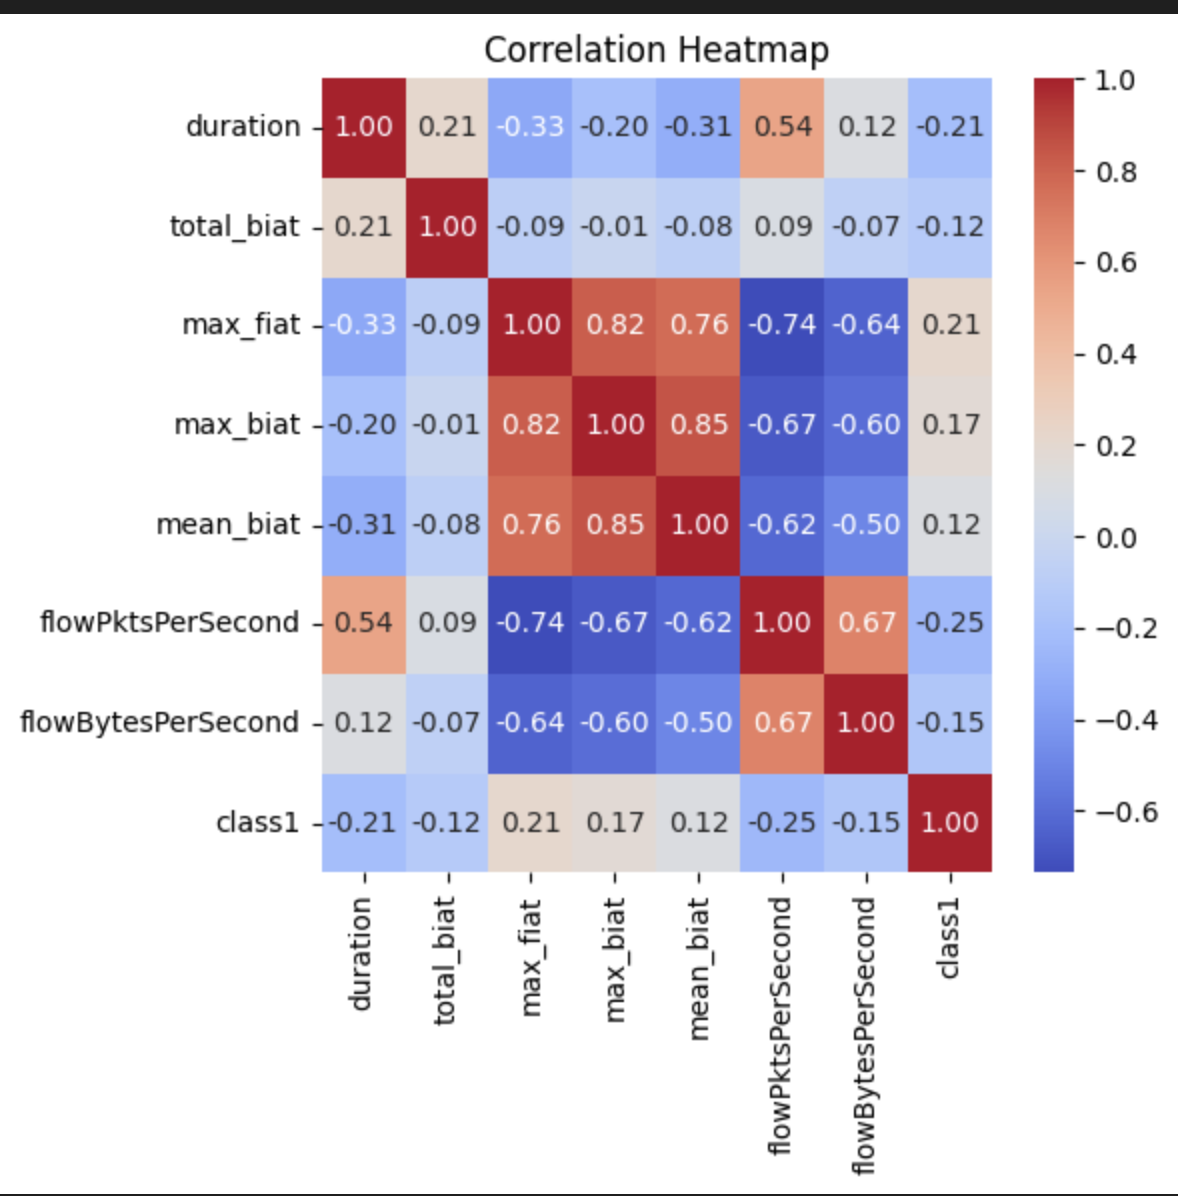
\includegraphics[width=0.8\textwidth]{Photo_Heatmap}
    \caption{상관관계 분석 결과}
\end{figure}

xgboost는 gradient boosting 알고리즘을 사용하여 트리 기반 모델을 학습하는 방법으로, 대량의 데이터셋을 처리하는 데에 강점을 가지고 있습니다.
또한, xgboost는 다양한 하이퍼파라미터를 조정할 수 있기 때문에 모델의 성능을 높일 수 있는 가능성이 높습니다.
저희는 xgboost 모델을 사용하여 VPN을 사용하지 않는 클라이언트의 트래픽을 분류하는 모델을 학습하였습니다.
Figure 3는 학습 결과를 나타내고 있습니다. Model의 Accuracy는 0.94로 충분히 높은 성능을 보였습니다.

\begin{figure}[h!]
    \centering
    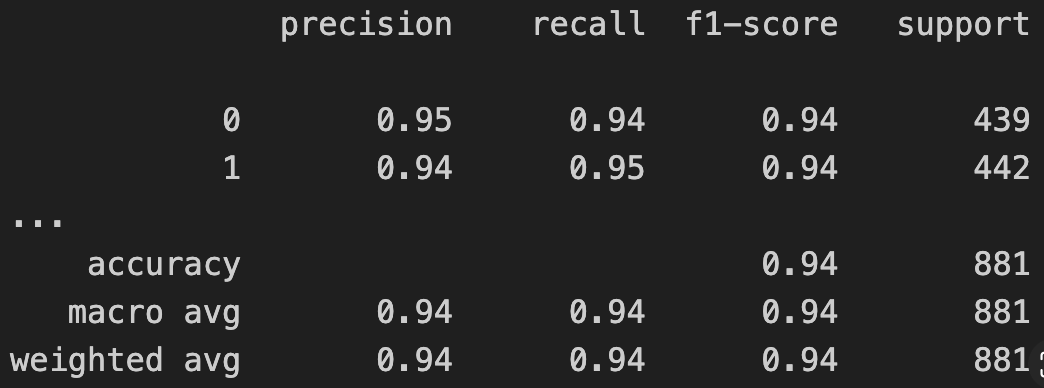
\includegraphics[width=0.8\textwidth]{Photo_Result} % 이미지 파일 이름
    \caption{모델 학습 결과}
\end{figure}

\section{\textit{What we will do}}
이제 본격적으로 저희의 연구 주제인 네트워크 트래픽 최적화 알고리즘을 고안하는 단계에 들어가고자 합니다.
개발한 분류 모델을 직접적으로 활용할 수 있는, VPN을 사용하지 않는 클라이언트의 트래픽을 우선적으로 처리하는 알고리즘을 고안해 볼 수 있을 것입니다.
이것 말고도 로드 밸런싱 알고리즘을 고안해 볼 수 있을 것입니다.
로드 밸런싱 알고리즘은 네트워크 트래픽을 여러 서버에 분산시켜서 서버의 부하를 줄이고, 네트워크 성능을 향상시키는 방법입니다.
이미 존재하는 다양한 로드 벨런싱 알고리즘을 분석하고, 저희의 연구 주제에 맞게 개선할 수 있는 방법을 찾아볼 수 있을 것입니다.

\end{document}